\chapter{Generic Data Structures}
\label{ch:generic}

\newcommand{\lecnum}{14}
%\newcommand{\lectitle}{Generic Data Structures}
\newcommand{\lecturer}{Rob Simmons, Iliano Cervesato}

\chapterTAGS{dictionary, function-pointer, genericity, hashing, interface, memory-model, queue, safety, void-star}
\maketitle

\begin{preamble}
\noindent
Our story about client interfaces in the previous chapter was
incomplete.  We were able to use client interfaces to implement queues
and hash tables that treat the client's types as abstract
(\lstinline'elem' for queues and sets, \lstinline'key' and
\lstinline'entry' for dictionaries), but any given program could only
have a \emph{single} type of keys, a \emph{single} way of hashing.

To solve these problems, we will have to move beyond the C0 language
to a language we call C1.  C1 gives us two important features that
aren't available in C0.  The first new feature is a \emph{void
  pointer}, which acts as a generic pointer.  The second new feature
is \emph{function pointers}, which allow us to augment hash
dictionaries with \emph{methods}, an idea that is connected to Java
and object-oriented programming.

Starting in this chapter, we will be working in an extension of C0
called C1.  To get the \lstinline'cc0' compiler to recognize C1, you
need to use files with a \lstinline'.c1' extension. Coin does not
currently accept C1.
\end{preamble}

\begin{gram}[Learning Goals]
Relating to our learning goals, we have
\begin{description}
\item[Computational Thinking: ]%
  Structs with function pointers that can be used to modify the data contained
  within the struct is an important idea from object oriented programming.

\item[Algorithms and Data Structures: ]%
  We will revisit the idea of hash dictionaries in a new setting.

\item[Programming: ]%
  We explore void pointers and function pointers, which are necessary
  for creating truly generic data structures in C0/C1.
\end{description}
\end{gram}


\newpage
\section{Generic Pointers: \lstinline'void*'}
\label{sec:generic:void_star}
\TAGS{genericity, safety, void-star}

We start by reexamining our queue data structure from last chapter.
Then, the library manipulated data of type \lstinline'elem' which the
client had to provide beforehand by a line like
\begin{lstlisting}[language={[C0]C}]
typedef string elem;    // supplied by client
\end{lstlisting}
One drawback of this is that the client program can only use a single
queue type --- queues of strings in this case.  The client can use
multiple queues of strings but not a queue of strings and a queue of
\lstinline'int''s for example.  If we need to do so, we have to make a
copy of the queue library, renaming all its functions and types.

To avoid this, we need to abandon C0 and make use of a feature of the
C1 language, the \emph{void pointer} (written \lstinline'void*').  C1
extends C0 with this and a few other features we will examine later in
this chapter.

A variable \lstinline'p' of type \lstinline'void*' is allowed to hold
a pointer to \emph{anything}.  Any pointer \lstinline'p' can be turned
into a void pointer by a \emph{cast}, written \lstinline'(void*)p':
\begin{lstlisting}[language={[C0]C}]
int*  ip = alloc(int);
void* p1 = (void*)ip;
void* p2 = (void*)alloc(string);
void* p3 = (void*)alloc(struct produce);
void* p4 = (void*)alloc(int**);
\end{lstlisting}
Because of this, void pointers are also called \emph{generic pointers}.

When we have a void pointer, we can turn it back into the type it came from
by casting in the other direction:
\begin{lstlisting}[language={[C0]C}]
int* x = (int*)p1;
string x = *(string*)p2;
\end{lstlisting}
This is the only operation we are allowed to perform on a void
pointer.  In particular, void pointers do not support dereferencing:
\lstinline'*p1' would give us back a \lstinline'void' which is not a
type at all --- it is just a marker to indicate that a function does
not return a value.  Thus, the name ``void pointer'' and the notation
\lstinline'void*' are terrible!  (But that's what they are called in
C.)  In C1, a cast can never appear on the left-hand side of an
assignment.

At run time, a non-\lstinline'NULL' void pointer has a \emph{tag}: casting
incorrectly, like trying to run \lstinline'(int*)p2' in the example above,
is a \emph{safety violation}: it causes a memory error just like a
\lstinline'NULL' dereference or array-out-of-bounds error.

These tags make void pointers a bit like values in Python: a void
pointer carries the information about its true pointer type, and an
error is raised if we treat a pointer to an integer like a pointer to
a string or vice versa.  Inside contracts, we can check that type with
the \lstinline'\hastag(type,p)' function:
% \begin{lstlisting}[language={[C0]C}]
% //@assert \hastag(int*, p1);
% //@assert \hastag(string*, p2);
% //@assert \hastag(int***, p4);

% //@assert !\hastag(string*, p1);
% //@assert !\hastag(int**, p1);
% //@assert !\hastag(int***, p1);
% \end{lstlisting}
\begin{lstlisting}[language={[C0]C}, belowskip=0pt]
//@assert \hastag(int*, p1);
//@assert \hastag(string*, p2);
//@assert \hastag(int***, p4);

//@assert !\hastag(string*, p1);
\end{lstlisting}%%% For some reason, doesn't work otherwise
\begin{lstlisting}[language={[C0]C}, aboveskip=0pt]
//@assert !\hastag(int**, p1);
//@assert !\hastag(int***, p1);
\end{lstlisting}
Like \lstinline'\length' for example, \lstinline'\hastag' cannot be used outside of contracts.

One quirk: since \lstinline'NULL' has any pointer type, calling
\lstinline'\hastag(type, p)' on a \lstinline'void*' variable \lstinline'p'
containing \lstinline'NULL' always returns \lstinline'true'.  This
lets us do slightly strange things like this without any error:
\begin{lstlisting}[language={[C0]C}]
void* p = NULL;
void* x = (void*)(int*)(void*)(string*)(void*)(struct wcount*)p;
\end{lstlisting}


\section{Generic Data Structures --- II}
\label{sec:generic:generic_libraries}
\TAGS{genericity, queue, void-star}

We can make our queue library fully generic by simply choosing
\lstinline'void*' as the type \lstinline'elem'.  Therefore, the only
change to the library code is to provide this one-line definition:
\begin{lstlisting}[language={[C0]C}]
typedef void* elem;
\end{lstlisting}

On the client side, using this now fully generic queue library is
somewhat more laborious.  For one, elements must be pointers.
Therefore the client cannot have a queue of integers: she shall turn
it into a queue of integer pointers.  Second, since the type
\lstinline'elem' is ultimately \lstinline'void*', she must cast her
data to \lstinline'void*' (or equivalently \lstinline'elem') before
enqueuing it, and then cast it back to \lstinline'int*' before
accessing the value of a dequeued element.  Here is a client code
snippet where she enqueues 42 into a new queue, and prints the value
at the front of the queue:
\begin{lstlisting}[language={[C0]C}]
  queue_t I = queue_new();
  int* x = alloc(int);     // must store in allocated memory
  *x = 42;
  enq(I, (void*)x);        // must cast to void*
  int* y = (int*)deq(I);   // must cast back before use
  printint(*y);
\end{lstlisting}
Now, the same program can also make use of a queue \lstinline'S' meant
to hold string (pointers).  It can in fact make use of arbitrarily
many queues, each containing data of a different type.

Nothing prevents a user from putting both \lstinline'int*''s and
\lstinline'string*''s in the same queue.  This is rarely advisable
however, since the client would need to be able to predict the type of
each dequeued element.

\section{Towards Generic Hash Dictionaries}
\label{sec:generic:generic_hash_dicts}
\TAGS{dictionary, genericity, hashing, interface, void-star}

Now that we know about generic pointers, let's apply them to the hash
dictionaries we developed in the last chapter.  Recall that they were
semi-generic, leaving the definition of the types \lstinline'entry' of
hash table entries and \lstinline'key' of keys to the client --- with
the result that a program could use a hash table that stored a single
type of entries.

The library interface simply declares \lstinline'entry' and
\lstinline'key' (now a pointer).  The changes are marked.
\begin{lstlisting}[language={[C0]C}]
typedef void* entry; // NEW!
typedef void* key;   // NEW!

/*** Client interface ***/
key  entry_key(entry x)                 // Supplied by client
/*@requires x != NULL; @*/
/*@ensures  \result != NULL; @*/ ; // NEW!
int  key_hash(key k)                    // Supplied by client
/*@requires k != NULL; @*/ ;  // NEW!
bool key_equiv(key k1, key k2)          // Supplied by client
/*@requires k1 != NULL \&\& k2 != NULL; @*/} ; // NEW!

/*** Library interface ***/
// typedef ______* hdict_t;

hdict_t hdict_new(int capacity)
/*@requires capacity > 0; @*/
/*@ensures \result != NULL; @*/ ;

entry hdict_lookup(hdict_t H, key k)
/*@requires H != NULL; @*/
/*@requires k != NULL; @*/ // NEW!
/*@ensures \result == NULL
        || key_equiv(entry_key(\result), k); @*/ ;

void hdict_insert(hdict_t H, entry x)
/*@requires H != NULL && x != NULL; @*/
/*@ensures hdict_lookup(H, entry_key(x)) == x; @*/ ;
\end{lstlisting}
Because keys are now pointers, we need to add \lstinline'NULL'-checks
anywhere a key is used.

\medskip%
The changes to the client code are more interesting.  We show the
updates to just the function \lstinline'entry_key' where they are most
pervasive.
\begin{lstlisting}[language={[C0]C}]
key entry_key(entry x)
//@requires x != NULL;
//@requires \hastag(struct wcount*, x); // NEW!
//@ensures \result != NULL \&\& \hastag(string*, \result); // NEW!
{
  string*{} k = alloc(string);
  *k = (struct wcount*)x->word;
  return (key)k;
}
\end{lstlisting}
The contracts refer to the abstract library types \lstinline'key' and
\lstinline'entry', but the client knows that in reality these types
are pointers to \lstinline'string''s and \lstinline'struct wcount''s
respectively.  This is noted as two calls to \lstinline'\hastag'.  Doing so
prevents mistakes like passing an argument of the wrong type or using
the result improperly --- recall that \lstinline'key' and
\lstinline'entry' are just nicknames to \lstinline'void*'.  Aside from
the now mandatory \lstinline'NULL'-check on the returned key, we need
to create space for it in allocated memory, cast the entry
\lstinline'x' to its original type, \lstinline'struct wcount*' in
order to be able to extract the word component we are using as key,
and then cast the result into a \lstinline'key' before returning.

Because the library contains the prototype of the client functions,
these functions do not need to be defined before their use in the
library functions.  Therefore the library file can now appear first on
the compilation command line, followed by the client files.  In fact,
there is no reason any more to split the client code into two files
and sandwich the library in between.

Using void pointers solves the unnatural dependency between client
functions and library code.  It doesn't make our hash dictionaries
fully generic however!

To understand why, try compiling a client program that uses two
different dictionaries, one for counting words as above, and a second
one with a different notion of entries and keys.  Although void
pointers can handle the different types, our program will necessarily
contain multiple definitions of the client functions, like
\lstinline'entry_key'.  Superficially, the compilation will fail
because it finds duplicate definitions of such functions.  More
deeply, our hash tables do not know which version to use when.  We
need to tell them.


\section{Memory Model}
\label{sec:generic:memory_model}
\TAGS{memory-model}

Up to now, we had a model of C0 execution where variables lived in
what we called \emph{local memory} and data created by means of
\lstinline'alloc_array' and \lstinline'alloc' were stored in
\emph{allocated memory}.  For example, here is a possible snapshot
during the execution of an program that uses our hash dictionaries:
\begin{center}
  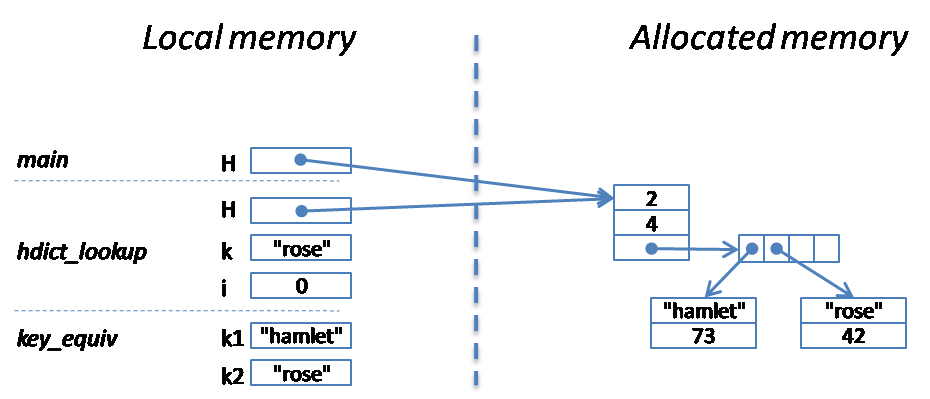
\includegraphics[width=0.9\textwidth]{img/memory-naive.png}
\end{center}

\begin{figure}[h!]
\begin{center}
  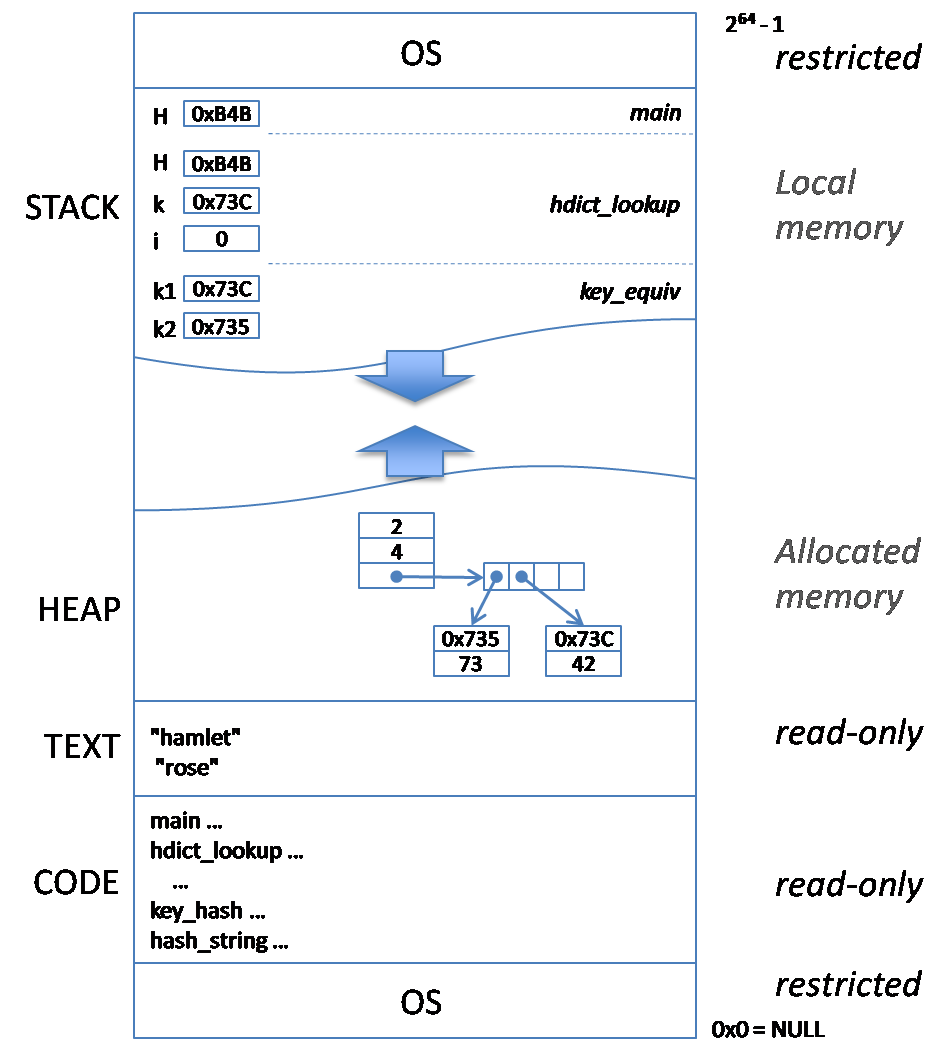
\includegraphics[width=0.9\textwidth]{img/memory.png}
\end{center}
\caption{A More Concrete Memory Model}
\label{fig:C0-memory}
\end{figure}

In reality, a computer contains a single entity we call \emph{memory},
and it needs to store many more things than our variables and the data
structures they point to.  A more realistic model of how memory is
organized is depicted in the figure~\ref{fig:C0-memory}.
We can think of memory as an array of bytes indexed by addresses ---
the very addresses coin reported when allocating arrays and pointers
(but now there are more).  Because addresses in C0 (and C1) have 64
bits, this array appears to have size $2^{64}$.  It is organized into
a number of \emph{segments}:
\begin{description}
\item[OS:] The two ends of this memory array belong to the operating
  system.  It uses these segments to hold its own data structures.
  A C0 program has no access to these areas --- they are
  \emph{restricted}.  It is convention to use address \lstinline'0x0'
  as \lstinline'NULL'.  It is an address after all, but one that we
  as programmers cannot do anything with.
\item[Stack:] What we referred to so far as ``local memory'' is
  normally called the \emph{stack}.  If we think about it, each time
  we enter a function, its local variables come into existence, and
  they go out of existence when we exit this function.  The nested
  nature of function calls make local memory behave like a stack.  The
  stack grows downward from the OS area at the end of the memory
  array.
\item[Heap: ] Our old ``allocated memory'' is typically called the
  \emph{heap}.  As we allocate new data structures, it grows towards
  the stack.
\item[Text: ] Next comes the \emph{text} segment which contains all
  the string literals present in our program.  So far, we had the
  illusion that strings were stored in variables and in locations in
  allocated memory.  In reality, these are addresses in the text area.
\item[Code: ] The last segment we shall concern ourselves with is
  where the compiled code of our program resides.  The code had to
  live somewhere after all!
\end{description}


\section{Function Pointers}
\label{sec:generic:function_pointers}
\TAGS{function-pointer}

The language C1 provides an operator, written \lstinline'&' and
pronounced ``\emph{address-of}'', to grab the address in the code
segment that corresponds to a function in a program.  For example,
\lstinline'&hash_string' is the address where the binary code for the
function \lstinline'hash_string' is located.  The address-of
operator can only be applied to functions in C1, although its use is
much more general in C\@.

Now that we can get a hold of a function address, we would like to
assign it to a variable, for example by writing %
\lstinline'F = &hash_string' and then apply \lstinline'F' to some
input.  But every variable shall have a type.  What is the type of
\lstinline'F'?  The \emph{type of a function} describes the number,
position and type of its input parameters and its output type.  In C1,
we declare a function type by just adding the word \lstinline'typedef'
in front of its prototype.  Since the prototype of
\lstinline'hash_string' is
\begin{lstlisting}[language={[C0]C}]
int hash_string(string s);
\end{lstlisting}
we write the type of this function as
\begin{lstlisting}[language={[C0]C}]
typedef int hash_string_fn(string s);
\end{lstlisting}
By convention, we use \lstinline'_fn' as a suffix for function types,
just like we used \lstinline'_t' as a suffix for client-side abstract
data types.  Note that \lstinline'hash_string_fn' is not the type of
just \lstinline'hash_string', but of every function that takes a
\lstinline'string' as input and returns an \lstinline'int' --- for
example the predefined string function \lstinline'string_length' has
this type too!

We can now declare the variable \lstinline'F' and assign
\lstinline'&hash_string' to it as follows:
\begin{lstlisting}[language={[C0]C}]
hash_string_fn* F = &hash_string;
\end{lstlisting}
Note that \lstinline'F' is pointer to a \lstinline'hash_string_fn',
which is consistent with the view that it contains an address in
memory.  \lstinline'F' is a \emph{function pointer}.  Because C1
variables, like C0 variables, can only hold values of small types,
we cannot assign directly a function to a variable --- thus
\begin{lstlisting}[language={[C0]C}]
hash_string_fn F = hash_string;   // NOT ALLOWED
\end{lstlisting}
is illegal.

We don't create function pointers by dynamically allocating them the
way we do structs: all the functions we could possibly have in our
program are already known when we compile the program, and we grab
them using \lstinline'&'.

To call the function assigned to a function pointer, we dereference
the pointer and then supply arguments.  For example
\begin{lstlisting}[language={[C0]C}]
(*F)("hello")
\end{lstlisting}
The parentheses around \lstinline'*F' are important:
\lstinline'*F("hello")' would have the effect of attempting to apply
\lstinline'F' to \lstinline'"hello"' and then dereference the result
--- the compiler will dutifully inform us that his makes no sense.

Like all other pointers, function pointers can be \lstinline'NULL', and it
is a safety violation to dereference a \lstinline'NULL' function pointer.


\section{Generic Data Structures --- III}
\label{sec:generic:libraries_function_pointers}
\TAGS{dictionary, function-pointer, genericity, hashing, interface, void-star}

Function pointers give us the mechanism for telling the library which
client functions it should use at any point in the program.  Whenever
a hash dictionary function relies on client functions, we will provide
it with pointers to the right functions.

Our first step is to convert the client function prototypes in the
library to function types:
\begin{lstlisting}[language={[C0]C}]
typedef key entry_key_fn(entry x)
         /*@requires x != NULL; @*/
         /*@ensures \result != NULL; @*/ ;
typedef int key_hash_fn(key k)
          /*@requires k != NULL; @*/ ;
typedef bool key_equiv_fn(key k1, key k2)
          /*@requires k1 != NULL; @*/
          /*@requires k2 != NULL; @*/ ;
\end{lstlisting}
Recall that this amounts to simply prefixing them with the keyword
\lstinline'typedef'.

Next, we need to decide \emph{how} to provide the client functions to
the library code.  A first idea is to simply pass them as additional
parameters, for example as in the following header
\begin{lstlisting}[language={[C0]C}]
entry hdict_lookup(hdict* H, key k,
                   entry_key_fn* to_key, key_equiv_fn* equiv)
\end{lstlisting}
Although possible, this approach pushes the burden of using the right
functions to the client, for each use of a library function.  In a
program that makes use of multiple hash dictionaries, it is
easy to make mistakes --- after all, every key equivalence function
will have type \lstinline'key_equiv_fn'!

A better approach is for the client to specify once and for all which
functions to use when creating the hash table, via
\lstinline'hdict_new', and storing these functions in the type that
defines the hash table.  To do this, we need to extend
\lstinline'struct hdict_header' with three fields of function pointer
type:
\begin{lstlisting}[language={[C0]C}]
typedef struct hdict_header hdict;
struct hdict_header {
  int size;             // 0 <= size
  chain*[] table;       // \length(table) == capacity
  int capacity;         // 0 < capacity
  entry_key_fn key;     // != NULL     // NEW!
  key_hash_fn hash;     // != NULL     // NEW!
  key_equiv_fn equiv;   // != NULL     // NEW!
};
\end{lstlisting}
Note the requirements that these pointers be non-\lstinline'NULL'.
These requirements will need to be reflected in the data structure
invariant functions \lstinline'is_hdict', which we omit.

The new fields get populated by the library function
\lstinline'hdict_new', which is updated as follows:
\begin{lstlisting}[language={[C0]C}]
hdict* hdict_new(int capacity, entry_key_fn* entry_key,
                 key_hash_fn* hash, key_equiv_fn* equiv)
//@requires capacity > 0;
//@requires entry_key != NULL && hash != NULL && equiv != NULL;
//@ensures is_hdict(\result);
{
  hdict* H = alloc(hdict);
  H->size = 0;
  H->capacity = capacity;
  H->table = alloc_array(chain*, capacity);
  H->key   = entry_key;         // NEW!
  H->hash  = hash;              // NEW!
  H->equiv = equiv;             // NEW!
  return H;
}
\end{lstlisting}
Every time we create a hash dictionary, the new fields will
contain pointers to the appropriate functions.  Therefore, a hash
dictionary now contains some of the functions that are used to
manipulate it.  This is one of the fundamental ideas underlying
\emph{object-oriented} programming.  Objects are data fields bundled
together with functions that operate on them.  These functions are
called \emph{methods} in object-oriented languages like Java.

At this point, all it takes to make our hash dictionary library fully
generic is to replace calls to \lstinline'key_equiv' to
\lstinline'(*H->equiv)' throughout the implementation, where
\lstinline'H' refers to the current hash dictionary.  Note that the
operator precedence rules of C1 parse \lstinline'(*H->equiv)' as
\lstinline'(*(H->equiv))'.

We can actually do slightly better, and at the same time isolate uses
of C1's rather cumbersome syntax for method calls (compared to
object-oriented languages).  We avoid having lots of calls that use
the counter-intuitive notation \lstinline'(*H->equiv)(x,y)' by writing
a helper function conveniently called \lstinline'key_equiv' --- or
original name for this client function --- so we can write calls that
look like \lstinline'key_equiv(H, x, y)'.  We do the same for the
other two client functions.

We show the resulting code for \lstinline'hdict_lookup' as an example:
\begin{lstlisting}[language={[C0]C}]
entry hdict_lookup(hdict* H, key k)
//@requires is_hdict(H) && k != NULL;
/*@ensures \result == NULL
        || key_equiv(H, entry_key(H, \result), k); @*/
{
  int i = index_of_key(H, k);
  for (chain* p = H->table[i]; p != NULL; p = p->next) {
    if (key_equiv(H, entry_key(H, p->data), k))
      return p->data;
  }
  return NULL;
}
\end{lstlisting}

Before moving to the client side, we need to revisit the library
interface.  Recall that we could write the prototype of
\lstinline'hdict_lookup' as
\begin{lstlisting}[language={[C0]C}]
entry hdict_lookup(hdict_t H, key k)
/*@requires H != NULL && k != NULL; @*/
/*@ensures \result == NULL
        || key_equiv(entry_key(\result), k); @*/ ;
\end{lstlisting}
Now, the functions \lstinline'key_equiv' and \lstinline'entry_key' are
internal to the implementation, and therefore they should not be made
available to the client.  Unraveling \lstinline'key_equiv' into
\lstinline'(*H->equiv)' will not work either because it too exposes
the internals of the implementation.  Our only choice is to do without
this postcondition.  The interface prototype of
\lstinline'hdict_lookup' is therefore
\begin{lstlisting}[language={[C0]C}]
entry hdict_lookup(hdict_t H, key k)
/*@requires H != NULL && k != NULL; @*/ ;
\end{lstlisting}

The upgrade we just made to the library has minimal effects on the
client side.  She simply needs to give new names to the client
interface functions.  She will also need to pass these functions each
time she creates a new hash dictionary using \lstinline'hdict_new'.

\clearpage
\section{Exercises}
\label{sec:generic:exercises}

\begin{flex}
\begin{exercise}%[\opt{sample solution on page~\pageref{ex:fn_void_list-solved}}]
\label{ex:fn_void_list}
One way to store elements of different type in a linked list is to
make it generic, giving its \lstinline'data' field type
\lstinline'void*'.  But then we won't be able to remember the actual
type of the element when we need to use it.  We use the additional
field \lstinline'tag' to keep track of it.
\begin{lstlisting}[language={[C0]C}]
typedef struct list_node genlist;
struct list_node {
  void* data;
  string tag;   // records the actual type of data
  genlist* next;
};
\end{lstlisting}
Assume that the only types we want to store in such a list are
integers and strings, with tags \lstinline'"an_int"' and
\lstinline'"a_string"' respectively.  Write a function that, given a
generic linked list, prints each of its elements on a separate line.
Include contracts as appropriate.  If it encounters an unknown tag, it
should call \lstinline'error' with a description of the problem.
\end{exercise}

\begin{solution}\opt{\textbf{of exercise~\ref{ex:fn_void_list}}}
\label{ex:fn_void_list-solved}
\begin{lstlisting}[language={[C0]C}]
void print_genlist(genlist* L) {
  for (genlist* p = L; p != NULL; p = p->next) {
    if (string_equal(p->tag, "an_int")) {
      //@assert \hastag(int*, p->data);
      printint(*(int*)p->data);
      println("");
    } else if (string_equal(p->tag, "a_string")) {
      //@assert \hastag(string*, p->data);
      println(*(string*)p->data);
    } else {
      print(p->tag);
      error(" is an unknown tag");
    }
  }
}
\end{lstlisting}
\end{solution}
\end{flex}


\begin{flex}
\begin{exercise}%[\opt{sample solution on page~\pageref{ex:fn_compose-solved}}]
\label{ex:fn_compose}
Define the function type \lstinline'int2int_fn' of all functions that
take an integer as input and return an integer.  Then, implement the
following two functions
\begin{lstlisting}[language={[C0]C}]
int compose(int2int_fn* f, int2int_fn* g, int x)
/*@requires f != NULL && g != NULL; @*/ ;

int pipeline(int2int_fn*[] F, int n, int x)
/*@requires \length(F) == n; @*/ ;
\end{lstlisting}
Given two mathematical functions $f$ and $g$ on the integers and an
integer $x$, the first implement applying the composition of $f$ and
$g$, often written $f \circ g$, to $x$.  Recall that $(f \circ g)(x) =
g(f(x)$.   The second applies all the functions in the
\lstinline'n'-element array \lstinline'F' to the integer
\lstinline'x', left to right.  If \lstinline'F' is empty, it shall
return \lstinline'x' unchanged.
\end{exercise}

\begin{solution}\opt{\textbf{of exercise~\ref{ex:fn_compose}}}
\label{ex:fn_compose-solved}
\begin{lstlisting}[language={[C0]C}]
typedef int int2int_fn(int x);

int compose(int2int_fn* f, int2int_fn* g, int x)
//@requires f != NULL && g != NULL;
{
  return (*f)((*g)(x));
}

int pipeline(int2int_fn*[] F, int n, int x)
//@requires \length(F) == n;
{
  int res = x;
  for (int i=0; i<n; i++)
  //@loop_invariant 0 <= i && i <= n;
  {
    res = (*(F[i]))(res);
  }
  return res;
}
\end{lstlisting}
\end{solution}
\end{flex}





% %%% This is a written exercises -- change to ask just about is_sorted
% \begin{flex}
% \begin{exercise}[\opt{sample solution on page~\pageref{ex:generic-binsearch-solved}}]
% \label{ex:generic-binsearch}
% Binary search works on a sorted array and relies on determining
% whether the element we are looking for is smaller, equal, or larger
% than the elements we are inspecting in the array.  We can make it
% generic by passing to it a comparison function, of type
% \lstinline'compare_fn', for this purpose and defining the type
% \lstinline'elem' of elements as \lstinline'void*':
% \begin{lstlisting}[language={[C0]C}]
% typedef void* elem;
% \end{lstlisting}
% Define the type \lstinline'compare_fn' and implement the specification
% function \lstinline'is_sorted' that checks if its input array is
% sorted according to a given comparison function, and
% \lstinline'binsearch' that implements binary search on a generic
% array.  Their prototypes are as follows:
% \begin{lstlisting}[language={[C0]C}]
% bool is_sorted(elem[] A, int lo, int hi, compare_fn* compare)
% /*@requires 0 <= lo  && lo <= hi && hi <= \length(A); @*/
% /*@requires compare != NULL; @*/ ;

% int search(elem x, elem[] A, int n, compare_fn* compare)
% /*@requires n == \length(A) && compare != NULL; @*/
% /*@requires is_sorted(A, 0, n, compare); @*/
% /*@ensures (\result == -1 && !is_in(x, A, 0, n, compare))
%         || (0 <= \result && \result < n &&
%            (*compare)(A[\result], x) == 0); @*/ ;
% \end{lstlisting}
% The specification function \lstinline'is_in(x, A, 0, n, compare)' checks
% that \lstinline'x' is in the array segment $[0, n)$ according to
% \lstinline'compare'.  You may assume it given, but feel free to implement
% it if you want an extra challenge.
% \end{exercise}

% \begin{solution}\opt{\textbf{of exercise~\ref{ex:generic-binsearch}}}
% \label{ex:generic-binsearch-solved}
% \begin{lstlisting}[language={[C0]C}]
% typedef int compare_fn(elem e1, elem e2)
% /*@ -1 <= \result && \result <= 1; @*/ ;

% bool is_sorted(elem[] A, int lo, int hi, compare_fn* compare)
% //requires 0 <= lo  && lo <= hi && hi <= \length(A);
% //requires compare != NULL;
% {
%   if (n <= 1) return true;

%   //@assert n >= 2;
%   elem x = A[0];
%   for (int i = 1; i < n; i++)
%   //@loop_invariant 1 <= i && i <= n;
%   {
%     if ((*compare)(x, A[i]) == 1) // x is larger than A[i]
%       return false;
%     x = A[i];
%   }
%   return true;
% }

% int search(elem x, elem[] A, int n, compare_fn* compare)
% //@requires n == \length(A) && compare != NULL;
% //@requires is_sorted(A, 0, n, compare);
% /*@ensures (\result == -1 && !is_in(x, A, 0, n))
%         || (0 <= \result && \result < n &&
%            (*compare)(A[\result], x) == 0); @*/
% {
%   int lo = 0;
%   int hi = n;

%   while (lo < hi)
%   //@loop_invariant 0 <= lo && lo <= hi && hi <= n;
%   {
%     int mid = lo + (hi - lo)/2;
%     //@assert lo <= mid && mid < hi;

%     int cmp = (*compare)(A[mid], x);
%     if (cmp == 0) return mid;
%     if (cmp < 0) {
%       lo = mid+1;
%     } else { //@assert cmp > 0;
%       hi = mid;
%     }
%   }
%   //@assert lo == hi;
%   return -1;
% }
% \end{lstlisting}
% \end{solution}
% \end{flex}



\printsolutions
% \clearpage
% \bibliographystyle{alpha}
% \bibliography{modal}
